\documentclass[inverse]{../slidedeck}
\newcommand*\thetitle{README}
\newcommand*\thesubtitle{vs. IEEE, RUP, SWEBOK, CMMI}
\sdTopLeft{@yegor256}
\sdBottomLeft{Lecture \#1: \thetitle{} \thesubtitle{}}
\begin{document}

\sdPrint{
  \sdTitle{\thetitle}{\thesubtitle}

  Lecture \#1 \br
  90 minutes
}

\sdClear

\sdSticker{Agenda}
\sdToc{Software vs. Interiors}\sdClick
\sdToc{IEEE 1016}\sdClick
\sdToc{SAD \@ RUP}\sdClick
\sdToc{TS \@ CMMI}\sdClick
\sdToc{SWEBOK}\sdClick
\sdToc{README}\sdClick
\sdToc{Books, Venues, C2A}

\sdClear
\sdStickerDelete
\sdTocNext
\sdPrint{\sdQuote{freeman}{Design encompasses all the activities involved in \ul{conceptualizing}, \ul{framing}, \ul{implementing}, \ul{commissioning}, and ultimately \ul{modifying} complex systems—not just the activity following requirements specification and before programming, as it might be translated from a stylized software engineering process.}{Peter Freeman and David Hart \br CACM vol. 47, no. 8, 2004}}

\sdClear
\sdPrint{\sdQuote{ieee-1016}{}{IEEE 1016-2009, \br IEEE Standard for Information Technology---Systems Design---Software Design Descriptions}}

\sdSticker{SDD}
\sdClear
\sdPrint{\sdBanner[green]{\large Software Design Description (SDD)}}

\sdClear
\sdMenu{Glossary}
\sdMenu{Languages}
\sdMenu{Stakeholders}
\sdMenu{Concerns}
\sdMenu{Viewpoints}
\sdMenu{Elements}
\sdMenu{Rationale}

% Glossary
\sdPrint{
  A \ul{request} is data package sent from a \ul{client} to a \ul{server}.\br
  A \ul{client} is a computer with a web browser.\br
  A \ul{server} is a computer with a software installed.\br
}\sdClick
\sdPrint{\sdBanner[green]{If I don't understand you, it's your fault!}}\sdClick
\sdPrint{\sdQR{https://www.yegor256.com/2015/03/16/technical-glossaries.html}}

% Languages
\sdClear
\sdMenuNext
\sdPrint{
  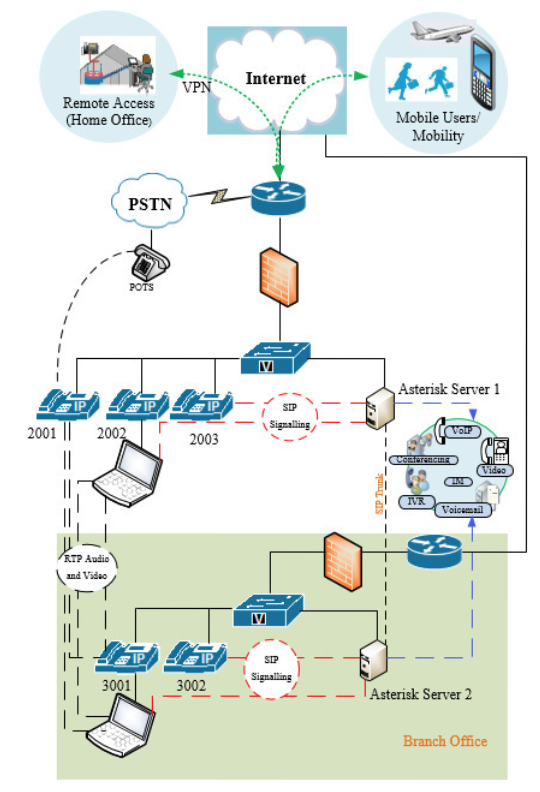
\includegraphics[width=0.4\textwidth]{bad-diagram}\par
  UML + visual-paradigm.com
}

% Stakeholders
\sdClear
\sdMenuNext
\sdPrint{\sdQuote{pmbok}{Identify Stakeholders is the process of identifying the people, groups, or organizations that could impact or be impacted by a decision, activity, or outcome of the project.}{A Guide to the Project Management \br Body of Knowledge (PMBOK\textregistered Guide), \br Project Stakeholder Management \br Knowledge Area}}

% Concerns
\sdClear
\sdMenuNext
\sdPrint{Functional \br and \br Non-Functional Requirements}

% Viewpoints
\sdClear
\sdMenuNext
\sdPrint{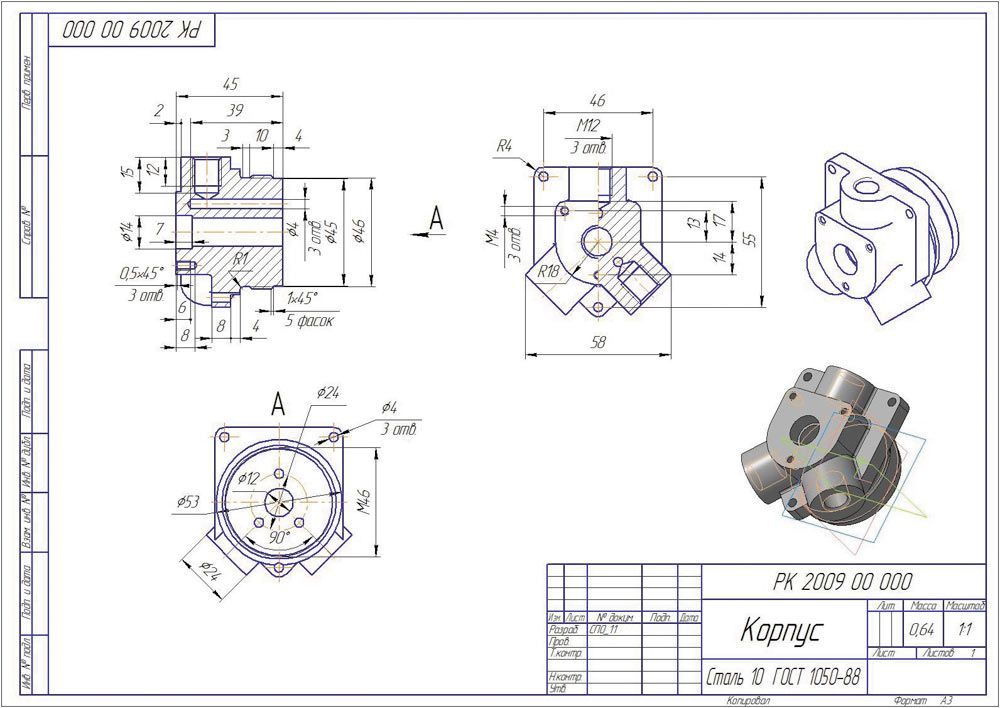
\includegraphics[width=0.5\textwidth]{viewpoint}}

% Elements
\sdClear
\sdMenuNext
\sdPrint{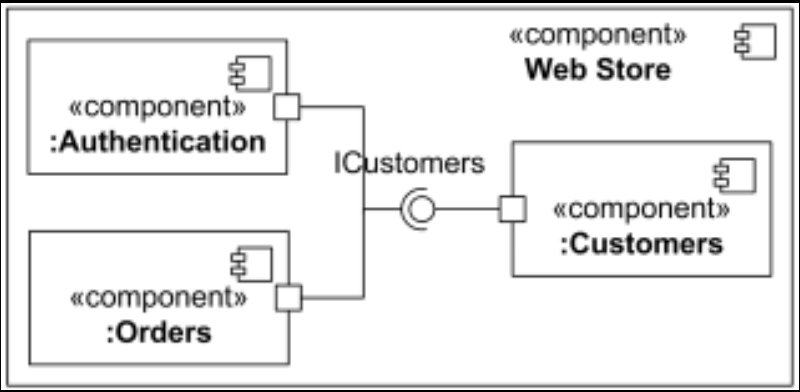
\includegraphics[width=0.3\textwidth]{element}}

% Rationale
\sdClear
\sdMenuNext
\sdPrint{\sdBanner[green]{\large Why MongoDB, why not MySQL?}}\sdClick
\sdPrint{
  Multi-Criteria Decision Making (MCDM)\\
  Architecture Tradeoff Analysis Method (ATAM)\\
  Decision Table\\
  Multi Factor Analysis\\
  Decision Matrix
}

\sdClear
\sdStickerDelete
\sdMenuDelete
\sdPrint{\sdQuote{cmmi}{Detailed design is focused on software product component development. The internal structure of product components is defined, data schemas are generated, algorithms are developed, and heuristics are established to provide product component capabilities that satisfy allocated requirements.}{CMMI for Development \br Capability Maturity Model Integration (CMMI\textregistered) \br Technical Solution (TS) Process Area}}

\sdClear

\end{document}
